\chapter[Cronograma]{Cronograma}
\label{chap:crono}

A imagem \ref{img:cronograma} mostra o cronograma das atividades realizadas durante a primeira parte do projeto. A segunda parte do projeto não possui cronograma ainda, pois não foram priorizadas as histórias de usuário que serão desenvolvidas.

\begin{figure}[H]
    \centering
    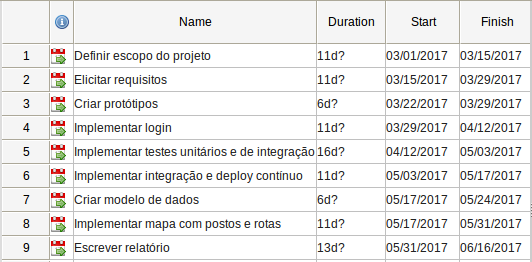
\includegraphics[scale=0.5]{figuras/cronograma_r1.png}
    \caption[Cronograma de atividades da primeira entrega.]{Cronograma de atividades da primeira entrega. Fonte: autores}
    \label{img:cronograma}
\end{figure}
